\documentclass{beamer}

\usepackage{graphicx}
\usepackage{mathtools}
\usepackage{mathrsfs}
\usepackage{fdsymbol}
\usepackage{hyperref}

%Information to be included in the title page:
\title{Hidden Variables}
\author{Congyuan Duan}
%\institute{School of Mathematics, Sun Yat-sen University}



\begin{document}

\frame{\titlepage}

\begin{frame}
    \frametitle{Contents}
    \tableofcontents
\end{frame}

\section{Interventional Sufficiency}

\begin{frame}
    \frametitle{Contents}
    \tableofcontents[currentsection]
\end{frame}

\begin{frame}
    \frametitle{Causally sufficient}
    \begin{itemize}
        \item[$\bullet$] A set of variables $\textbf{X}$ is usually said to be \textbf{causally sufficient} if there is no hidden
        common cause $C\notin \textbf{X}$ that is causing more than one variable in $\textbf{X}$. 
        \item[$\bullet$] A variable $C$ is a common cause of X and Y if there is a directed path
        from $C$ to $X$ and $Y$ that does not include $Y$ and $X$, respectively.
        \item[$\bullet$] Common causes are also called confounders.
    \end{itemize}
\end{frame}

\begin{frame}
    \frametitle{Interventional sufficiency}
    \centering{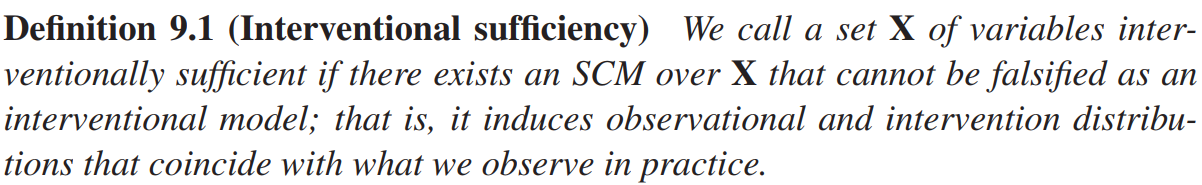
\includegraphics[scale=0.6]{fig1.png}}
    \begin{itemize} 
        \item[$\bullet$] Simpson's paradox shows that two variables are not causally sufficient if
        there exists a latent common cause, and in general these two variables are not interventionally sufficient either. \\
        \item[$\bullet$] There are also examples that the set of variables is interventionally sufficient but causally insufficient.
    \end{itemize}
\end{frame}

\begin{frame}
    \frametitle{Example}
    \begin{flushleft}
        Consider the following SCM
    \end{flushleft}
    \centering{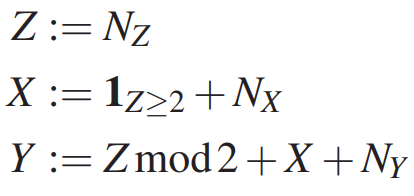
\includegraphics[scale=0.6]{fig2.png}}
    \begin{flushleft} 
        with $N_Z\sim U(\{0,1,2,3\})$ and $N_X,N_Y \overset{iid}\sim N(0,1)$. \\
    \end{flushleft}
    \centering{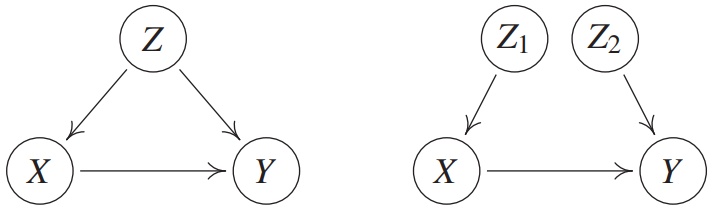
\includegraphics[scale=0.6]{fig4.png}}
    \begin{itemize}
        \item[$\bullet$] While variables $X$ and $Y$ are clearly causally insufficient, they interventionally sufficient.
        \item[$\bullet$] There cannot be a solely graphical criterion
        for determining whether a subset of the variables are interventionally sufficient.  
    \end{itemize}
\end{frame}

\begin{frame}
    \frametitle{Interventional sufficiency and causal sufficiency}
    \begin{flushleft}
        In general, we have the following relationship between causal and interventional
        sufficiency.
    \end{flushleft}
    \centering{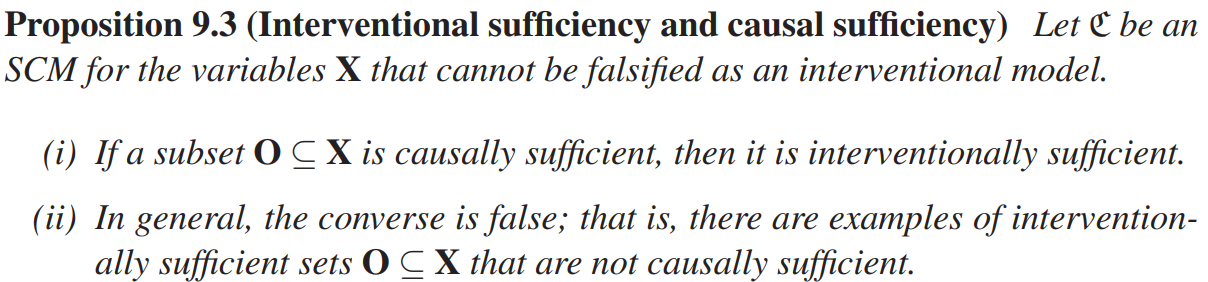
\includegraphics[scale=0.6]{fig3.png}}
\end{frame}

\section{Instrumental Variables}

\begin{frame}
    \frametitle{Contents}
    \tableofcontents[currentsection]
\end{frame}

\begin{frame}
    \frametitle{Instrumental Variables}
    \begin{flushleft}
        Consider a linear Gaussian SCM with graph
    \end{flushleft}
    \centering{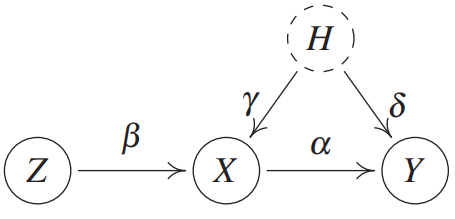
\includegraphics[scale=0.6]{fig15.png}}
    \begin{flushleft}
        Here, the coefficient $\alpha$ in the structural assignment
    \end{flushleft}
    \begin{align*}
        Y:= \alpha X + \delta H + N_Y
    \end{align*}
    \begin{flushleft}
        is the average causal effect. \\
        However, simply regressing Y on X results in a biased estimator.
    \end{flushleft}
\end{frame}

\begin{frame}
    \frametitle{Instrumental Variables}
    \centering{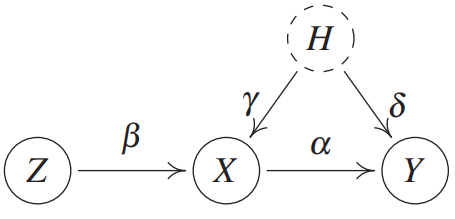
\includegraphics[scale=0.6]{fig15.png}}
    \begin{flushleft}
        Since $(H,N_X)$ is independent of $Z$, we can have
    \end{flushleft}
    \begin{align*}
        X:= \beta Z+\gamma H+N_X
    \end{align*}
    \begin{flushleft}
        Because of
    \end{flushleft}
    \begin{align*}
        Y:= \alpha X + \delta H + N_Y=\alpha(\beta Z) + (\alpha\gamma+\delta)H + N_Y
    \end{align*}
    \begin{flushleft}
        We can then consistently estimate $\alpha$ by regressing $Y$ on $\beta Z$. 
    \end{flushleft}
\end{frame}

\begin{frame}
    \frametitle{Instrumental Variables}
    \centering{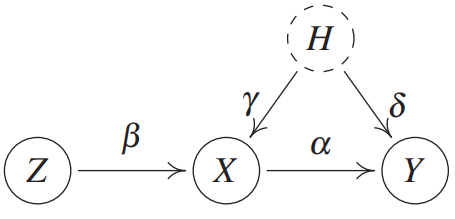
\includegraphics[scale=0.6]{fig15.png}}
    \begin{flushleft}
        We call a variable $Z$ in an SCM an instrumental variable for $(X,Y)$ if 
    \end{flushleft}
    \begin{itemize}
        \item[$\bullet$] $Z$ is independent of $H$.
        \item[$\bullet$] $Z$ is not independent of $X$.
        \item[$\bullet$] $Z$ effects $Y$ only through $X$.
    \end{itemize}
\end{frame}

\begin{frame}
    \frametitle{Instrumental Variables Under Potential Outcomes}
    \centering{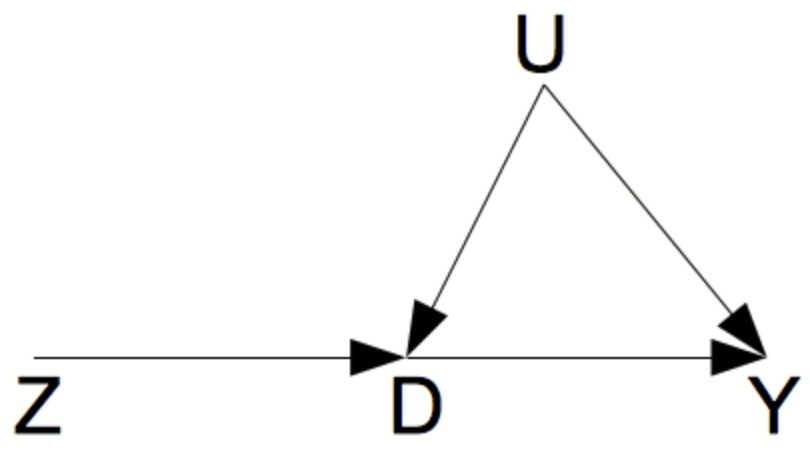
\includegraphics[scale=0.3]{fig16.png}}
    \begin{flushleft}
        Z:encouragement(randomly assigned) D:treatment Y:result
    \end{flushleft}
    \begin{itemize}
        \item[$\bullet$] As originally formulated, the potential outcomes $D_i(Z)$ and $Y_i(D)$ are fixed but unknown values partially
        observed through the assignment of treatments to units.
        \item[$\bullet$] We restricted both $Z$ and $D$ to have only two levels.
    \end{itemize}
\end{frame}

\begin{frame}
    \frametitle{Instrumental Variables Under Potential Outcomes}
    Assumptions:
    \begin{itemize}
        \item[$\bullet$] Random Assignment: $Z_i\Vbar \{D_i(1),D_i(0),Y_i(0),Y_i(1)\}$ 
        \item[$\bullet$] Exclusion Restriction: $Y(Z,D)=Y(Z^{\prime},D)$
        \item[$\bullet$] Nonzero Average Causal Effect: $E[D_i(1) - D_i(0)] $ is not equalto zero
        \item[$\bullet$] Monotonicity: $D_i(1)\geq D_i(0)$ for all $i=1,\cdots,N$
    \end{itemize}
    A variable $Z$ is an instrumental variable for the causal effect of $D$ on $Y$ if the above assumptions hold.
\end{frame}



\begin{frame}
    \frametitle{Instrumental Variables Under Potential Outcomes}
    \begin{flushleft}
        At the unit level, we have
    \end{flushleft}
    \centering{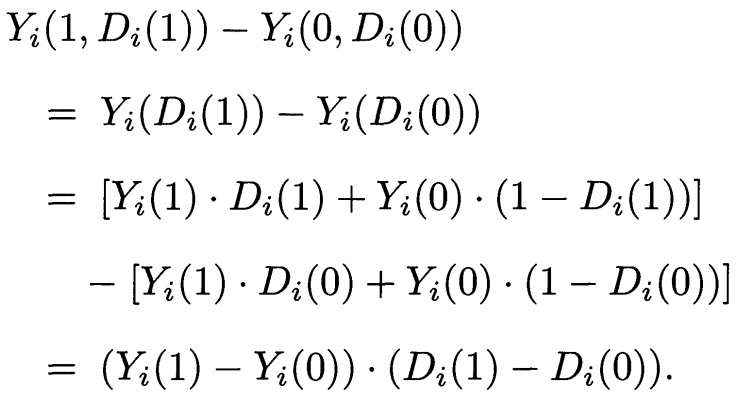
\includegraphics[scale=0.6]{fig17.png}}
    \begin{flushleft}
        Thus the causal effect of $Z$ on $Y$ for person $i$ is the product
        of (i)the causal effect of $D$ on $Y$ and (ii)the causal effect
        of $Z$ on $D$.
    \end{flushleft}
\end{frame}

\begin{frame}
    \frametitle{Instrumental Variables Under Potential Outcomes}
    \begin{flushleft}
        We can therefore write the average causal effect of $Z$ on $Y$ as:
    \end{flushleft}
    \centering{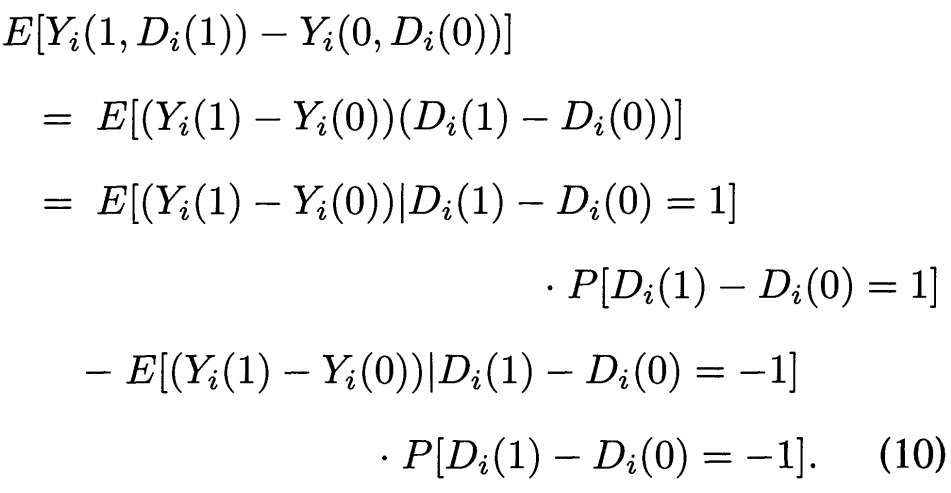
\includegraphics[scale=0.6]{fig18.png}}
    \begin{flushleft}
        Use the monotonicity assumption,
    \end{flushleft}
    \centering{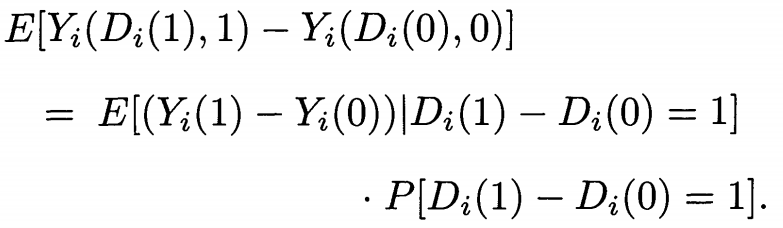
\includegraphics[scale=0.6]{fig19.png}}
\end{frame}

\begin{frame}
    \frametitle{Instrumental Variables Under Potential Outcomes}
    \begin{flushleft}
        The causal interpretation of the IV estimator is
    \end{flushleft}
    \begin{align*}
        \hat{\beta}^{IV}&= E[(Y_i(1)-Y_i(0))|D_i(1)-D_i(0)=1] \\
                        &= \frac{E[Y_i(D_i(1),1)-Y_i(D_i(0),0)]}{E[D_i(1)-D_i(0)]} \\
                        &= \frac{ACE(Z\rightarrow Y)}{ACE(Z\rightarrow D)}
    \end{align*}
    \begin{flushleft}
        We call this the Local Average Treatment Effect or Complier Average Causal Effect.
    \end{flushleft}
\end{frame}

\section{Conditional Independences and Graphical Representations}

\begin{frame}
    \frametitle{Contents}
    \tableofcontents[currentsection]
\end{frame}

\begin{frame}
    \frametitle{Difficulty}
    \begin{flushleft}
        We want to obtain identifiability results for an SCM $\mathfrak{C}$ over variables $\textbf{X}=(\textbf{O},\textbf{H})$ 
        that includes observed variables $\textbf{O}$ and hidden variables $\textbf{H}$. \\ 
        % In the case without hidden variables, we search over the space of DAGs and output a graph representing 
        % exactly the set of conditional independences found in the data. \\
        This comes with additional difficulties when searching over the space of DAGs with latent variables. 
    \end{flushleft}
    \begin{itemize}
        \item[$\bullet$] We do not know the size of $\textbf{H}$, so there is an infinite number of graphical candidates
        that we have to search over.
        \item[$\bullet$] The set of distributions that are Markovian and faithful with respect to
        a DAG forms a curved exponential family, which justifies the use of the BIC. The set of distributions that are Markovian 
        and faithful with respect to a DAG with latent variables, however, does not.
    \end{itemize}
    %或许加一句,P178倒数第二段的话?
\end{frame}

\begin{frame}
    \frametitle{Difficulty}
    \begin{flushleft}
        Can we assume that the entailed distribution $P_O$
        is Markovian and faithful with respect to a DAG without hidden variables instead?
    \end{flushleft}
    \begin{itemize}
        \item[$\bullet$] Representing the set of conditional independences with a DAG over the 
        observed variables can lead to causal misinterpretations.
        \item[$\bullet$] The set of distributions whose pattern of independences correspond to the d-separation statements in
        a DAG is not closed under marginalization.
    \end{itemize}
    \begin{figure}[htbp]
        \centering
        \begin{minipage}[t]{0.48\textwidth}
        \centering
        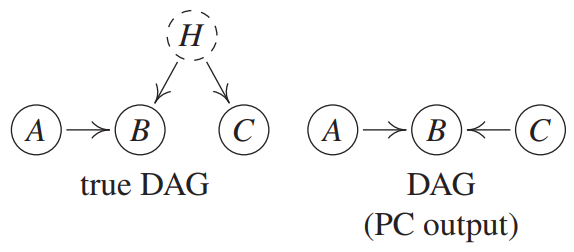
\includegraphics[scale=0.6]{fig5.png}
        \end{minipage}
        \begin{minipage}[t]{0.48\textwidth}
        \centering
        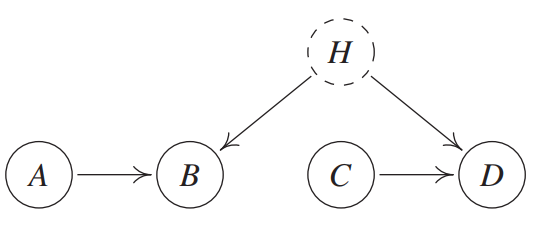
\includegraphics[scale=0.6]{fig6.png}
        \end{minipage}
    \end{figure}
\end{frame}

\begin{frame}
    \frametitle{Maximal Ancestral Graph}
    \begin{itemize}
        \item[$\bullet$] An inducing path relative to $L$ is a path
        on which every vertex not in $L$ (except for the endpoints) is a collider on the path and every collider
        is an ancestor of an endpoint of the path. 
        \item[$\bullet$] We refer to inducing paths relative to the empty set simply as inducing paths. 
        \item[$\bullet$] A directed cycle occurs in $\mathcal{G}$ when $Y\rightarrow X$ is in $\mathcal{G}$ and $X\in An(Y)$. 
        \item[$\bullet$] An almost directed cycle occurs when $Y\leftrightarrow X$ is in $\mathcal{G}$ and $X\in An(Y)$.  
    \end{itemize}
    \centering{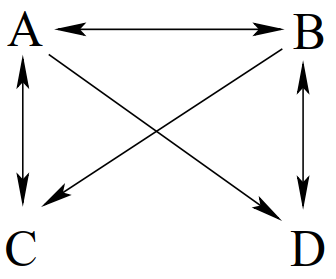
\includegraphics[scale=0.6]{fig8.png}}
\end{frame}

\begin{frame}
    \frametitle{Maximal Ancestral Graph}
    \centering{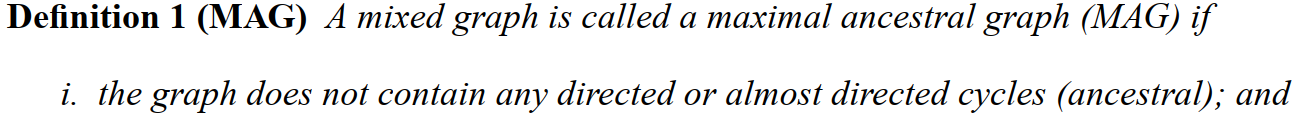
\includegraphics[scale=0.6]{fig9.png}}
    \centering{
\includegraphics[scale=0.6]{fig10.png}}
    \centering{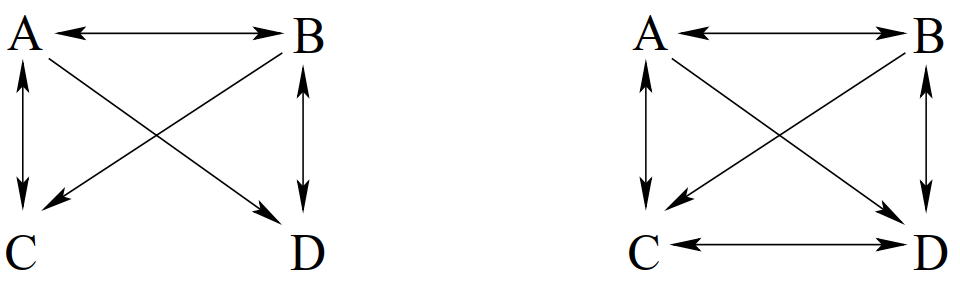
\includegraphics[scale=0.6]{fig11.png}}
    % \begin{flushleft}
    %     Before, we have used graphs to represent the structural relationships of SCMs. Here, the aim is to
    %     use graphs to represent constraints in the distribution induced by the SCM.
    % \end{flushleft}
\end{frame}

\begin{frame}
    \frametitle{m-separation}
    \begin{flushleft}
        It is straightforward to extend d-separation to mixed graphs.
    \end{flushleft}
    \centering{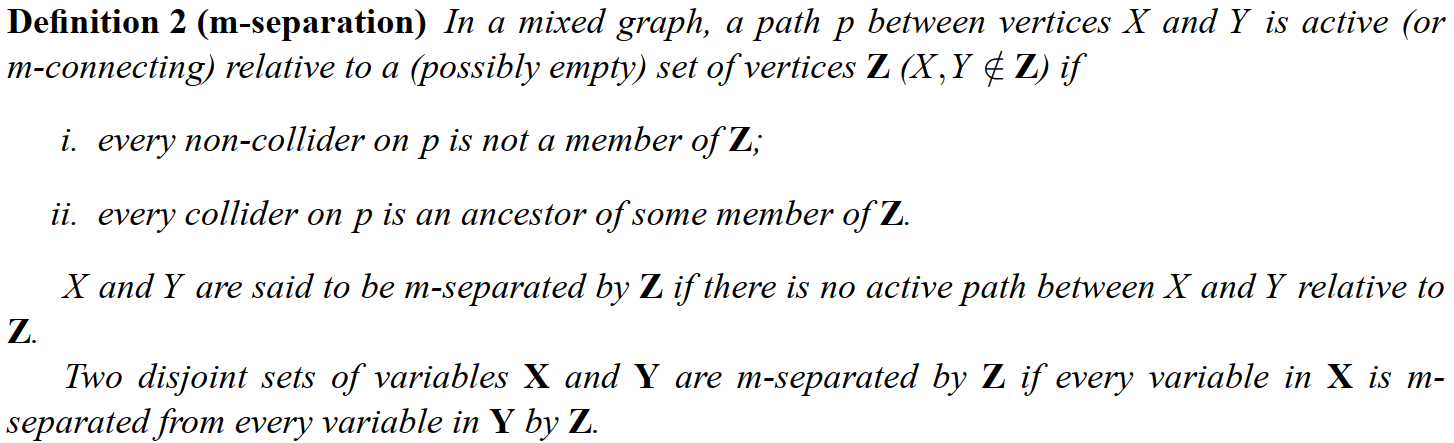
\includegraphics[scale=0.55]{fig12.png}}
    \begin{flushleft}
        This captures exactly the conditional independence relations entailed by a MAG according to the Markov condition.
    \end{flushleft}
\end{frame}

\begin{frame}
    \frametitle{Maximal Ancestral Graph}
    \begin{flushleft}
        MAGs represent the marginal independence models of DAGs: given any DAG $\mathcal{G}$ over $V=O\cup H$, there is a 
        MAG over O alone such that for any disjoint $X,Y,Z\subseteq O$, $X$ and $Y$ are d-separated by $Z$ in $\mathcal{G}$ 
        if and only if they are m-separated by $Z$ in the MAG. \\
        The following construction gives us such a MAG $M_{\mathcal{G}}$:
    \end{flushleft}
    \begin{itemize}
        \item[$\bullet$] For each pair of variables $A,B\in O$, $A$ and $B$ are adjacent in $M_{\mathcal{G}}$ if and only if there 
        is an inducing path between them relative to $H$ in $\mathcal{G}$. 
        \item[$\bullet$] For each pair of adjacent variables $A,B\in M_{\mathcal{G}}$, orient the edge as $A\rightarrow B$ if $A$ 
        is an ancestor of $B$ in $\mathcal{G}$; orient it as $A\leftarrow B$ if $B$ is an ancestor of $A$; orient it 
        as $A\leftrightarrow B$ otherwise.
    \end{itemize}
    \begin{flushleft}
        It can be shown that $M_{\mathcal{G}}$ is a MAG and represents the marginal independence model over $O$.
    \end{flushleft}
\end{frame}

\begin{frame}
    \frametitle{Maximal Ancestral Graph}
    \begin{itemize}
        \item[$\bullet$] Different causal DAGs may correspond to the same causal MAG.
        \item[$\bullet$] The MAG retains the causal relationships among the observed variables.
        \item[$\bullet$] Alternative definition: an ancestral graph is said to be maximal if, for every
        pair of non-adjacent nodes $X$, $Y$ there exists a set $Z$
        such that $X$ and $Y$ are m-separated conditional on $Z$.
    \end{itemize}
    Just as DAGs, different MAGs can entail the exact same constraints by the m-separation criterion. This motivates the following 
    representation of equivalence classes of MAGs. 
\end{frame}

\begin{frame}
    \frametitle{Partial Ancestral Graph}
    \centering{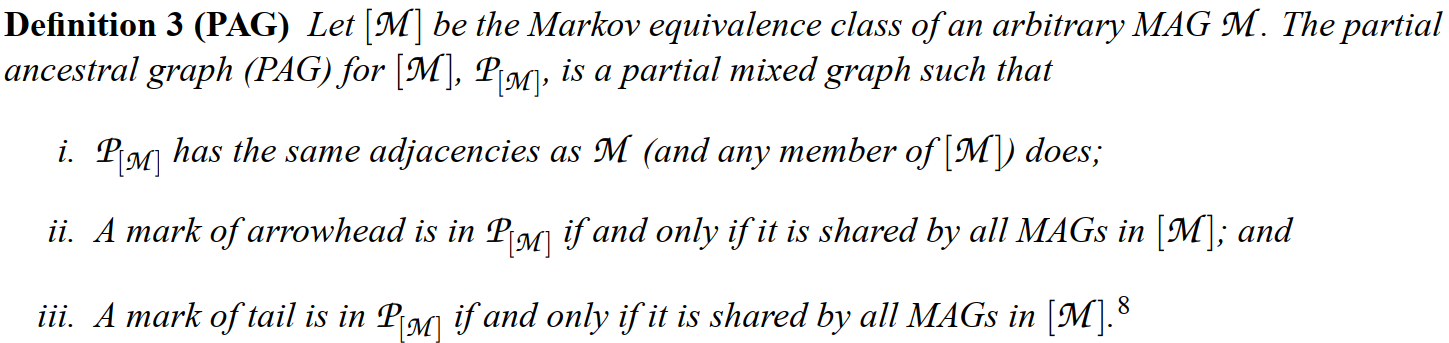
\includegraphics[scale=0.55]{fig13.png}}
    \begin{flushleft}
        In PAGs, edges can end with a circle, which represents both possibilities of an arrow's head and tail.
    \end{flushleft}
    \centering{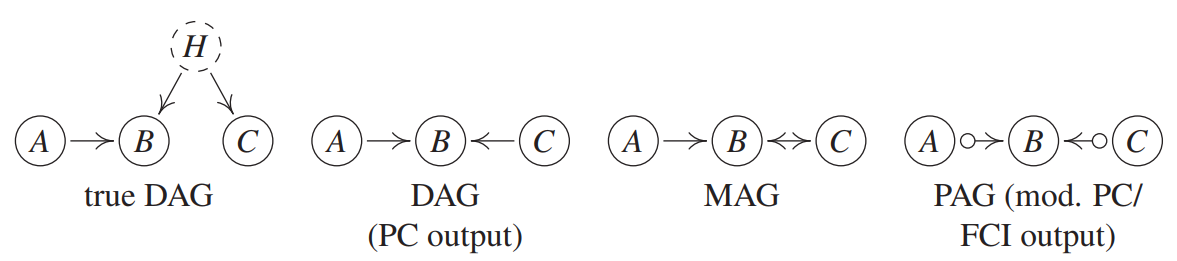
\includegraphics[scale=0.55]{fig14.png}}
\end{frame}

\begin{frame}
    \frametitle{Summary}
    \centering{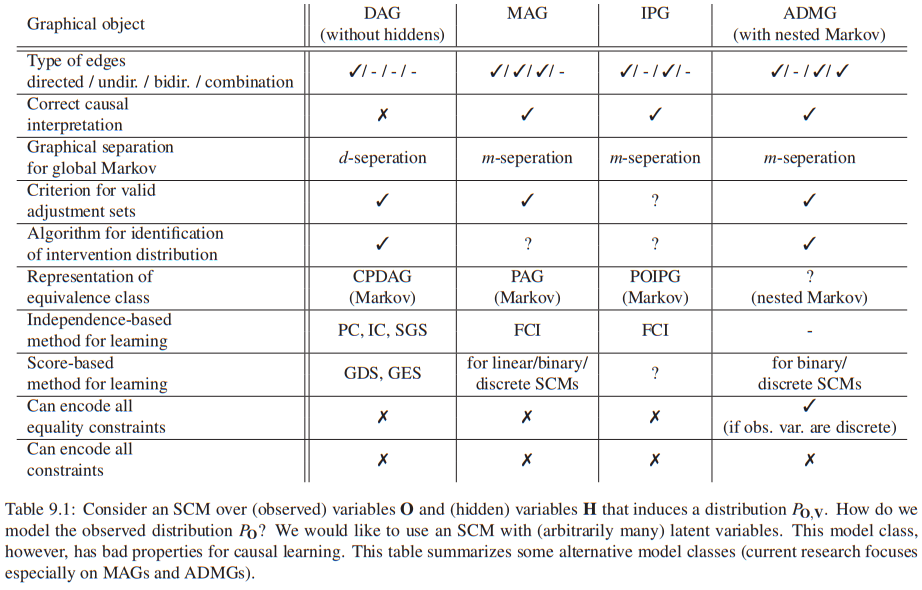
\includegraphics[scale=0.9]{fig7.png}}
\end{frame}

\begin{frame}
    \frametitle{Reference} 
    Angrist J D, Imbens G W, Rubin D B. Identification of causal effects using instrumental variables[J]. 
    Journal of the American statistical Association, 1996, 91(434): 444-455. \\
    Zhang J. Causal reasoning with ancestral graphs[J]. Journal of Machine Learning Research, 2008, 9: 1437-1474. \\
\end{frame}


\end{document}
